\chapter{\textit{Proposta}}\label{chp:proposta}

Portanto, pretendemos aplicar os diferentes métodos de aprendizado de máquina para detectar momentos de uma crise epilética. Ao final, iremos comparar a acurácia e a complexidade de cada método para esse determinado problema e discutir dos resultados obtidos.

Por fim, Vale salientar que o objetivo é fazer uma classificação binária em positivo ou negativo para um processo epiléptico dado diversos intervalos diferentes de tempo. O resultado esperado está representado na figura \ref{fig:binary_class}.

\begin{figure}[!h]
    \centering
    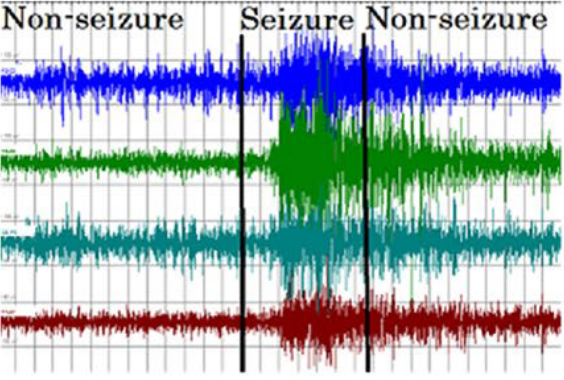
\includegraphics[width=0.4\textwidth]{figuras/binary_class.png}
    \caption{Classificação binária em uma amostra EEG}
    \label{fig:binary_class}
\end{figure}